%%This is a very basic article template.
%%There is just one section and two subsections.
\documentclass[12pt]{jsreport}
\usepackage[top=15truemm,bottom=15truemm,left=13truemm,right=13truemm]{geometry}
\usepackage{amsmath}
\usepackage{amssymb}
\usepackage{ascmac}
\usepackage{fancybox}
\usepackage[usenames]{color}
\usepackage{plext}
\usepackage{comment}
\usepackage{ulem}
\usepackage[dvipdfmx]{graphicx}

%%赤文字と赤下線
\newcommand{\ruline}[1]{\textcolor{red}{\underline{\textcolor{black}{#1}}}}
\newcommand{\red}[1]{\textcolor{red}{#1}}
%%改行用コマンド
\newcommand{\ret}{\\\quad}
\newcommand{\tret}[1]{\tag{#1}\\}
\newcommand{\ntret}{\notag\\}


\renewcommand{\thesection}{第\arabic{section}章}
\renewcommand{\thesubsection}{\arabic{section}.\arabic{subsection}}

\title{「TrimerX」要求仕様書}
\author{チーム「ちぃーず」\\05伊藤いちご\ 18金子航\ 24米華真典}
\date{}


\begin{document}
\maketitle
\newpage

\setcounter{tocdepth}{2}
\tableofcontents

\newpage

\setcounter{page}{1}

\section{概要}
本ソフト「TrimerX」は試験の答案やアンケートの集計をするための,画像のトリミングを主としたものです.トリミングしたものをまとめて見ることや答案の点数を入力・集計して平均点を計算することが可能です.

\newpage

\section{動作・開発環境}
本章では動作・開発環境に述べます,

\subsection{開発環境}

開発環境は以下の通りです.
\begin{itemize}
    \item Python\ 3.6.4
    \item PyQt\ 5.6.2
    \item OpenCV\ 3.4.1
\end{itemize}


\subsection{動作環境}
本ソフトは以下のOSで動作を確認しています.

\begin{itemize}
    \item macOS\ Sierra\ 10.12.6
\end{itemize}


\newpage


\section{ソフトウェアの構成}
本章では本ソフトの構成について述べます.本ソフトのトリミング機能は大きく分けて2種類になります.

用途に合わせてその機能を使い分けることによってデータの集計を円滑に行うことが可能です.

以下が本ソフトの機能の一覧です.
\begin{enumerate}
    \item メインウィンドウ
    \item トリミング
    \item データビュー
    \item データ入力・集計
    \item 画像の読み込み
\end{enumerate}

\newpage

\section{各機能の詳細}
本章では各機能の詳細を以下に述べます.

\subsection{メインウィンドウ}
図\ref{fig:MainWindow}は起動時に表示されるメインウィンドウのイメージです.
各ボタンをクリックすることでその機能を使用する事が出来ます.
終了する場合は左上の×ボタンからウィンドウを閉じます.
\begin{figure}[htbp]
  \centering
 \begin{minipage}{0.5\hsize}
  \begin{center}
   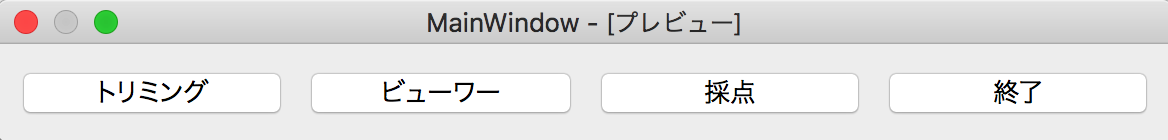
\includegraphics[width=70mm]{MainWindow.png}
  \end{center}
  \caption{メインウィンドウ}
  \label{fig:MainWindow}
 \end{minipage}
\end{figure}

\subsection{トリミング}
基本的なトリミング2種類を行えます.

\subsubsection{定型トリミング}

    主にアンケート用紙などの,大量のデータに対して位置を設定し連続的にトリミングを行います.
    切り取ったデータは種類ごとに同じファイルにまとめられ「データビュー」にて閲覧が可能となります.

\subsubsection{自由トリミング}


    主に自由記述型のテキストや解答用紙などに対して機能します.
    各解答に対しておおよその位置をマウスポインターによって指定することで,指定した位置に対して適切なトリミングを行います.
    一枚のプリントに対して連続的に位置を指定することができ,指定した順番によってファイル名も設定されます.

    自由トリミングの流れを図\ref{fig:FreeTrimFlow}に示します.

    \begin{figure}[htbp]
        \centering
        \begin{minipage}{1\hsize}
            \begin{center}
                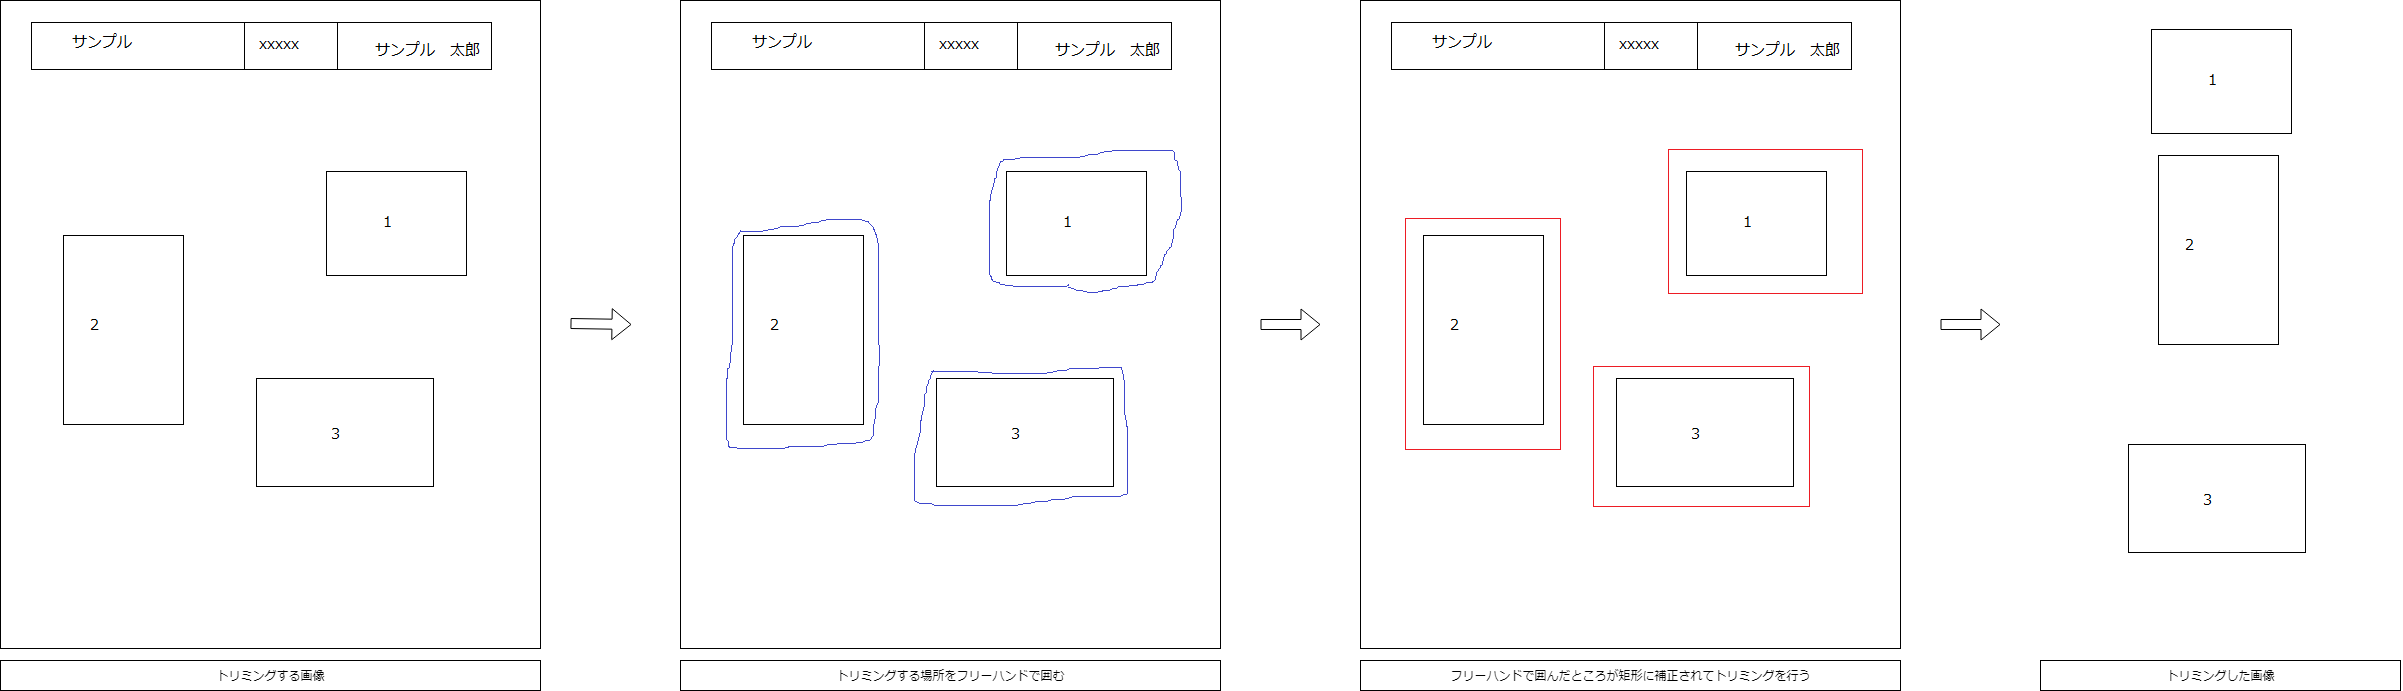
\includegraphics[width=150mm]{FreeTrimFlow.png}
            \end{center}
            \caption{自由トリミングの流れ}
            \label{fig:FreeTrimFlow}
        \end{minipage}
    \end{figure}

    図\ref{fig:FreeTrimFlow}のように自由トリミングはフリーハンドで囲ったところを包含する矩形でトリミングするようになっています


    具体的な手順としては
    \begin{enumerate}
        \item トリミングする画像を読み込む
        \item トリミングする箇所をフリーハンドで囲む
        \item フリーハンドの囲いを包含するような矩形を生成
        \item 生成した矩形データでトリミングを行う
    \end{enumerate}

    となっています,

\subsection{データビュー}
データが種類ごとに分別されており,閲覧することが可能です.
\subsection{データ入力・集計}
テストの解答に対して,問いごとに点数の入力を行えます.入力したデータはcsvファイルに出力され,平均点,合計点などの集計が可能です.
\subsection{画像の読み込み}
画像ファイル(.jpg)の読み込みはファイル毎に行われ,存在しているファイルによって属性が割り当てられます.





\newpage
\paragraph{改変履歴} \\
以下に改変履歴を記します.
\begin{table}[htb]
\caption{改変履歴}
\begin{center}
\begin{tabular}{|l|l|l|}
    \hline
    改変日 & 内容 & 担当 \\ \hline
    2018/07/11 & 目次の修正 & 米華 \\ \hline
    2018/07/12 & 第2章,第4章の初めにそれぞれの章の説明を追加 & 米華 \\ \hline
    2018/07/13 & ウィンドウイメージと各ボタンの機能についてを追加 & 金子 \\ \hline
    2018/07/13 & 自由トリミングの流れ図を追加 & 米華 \\ \hline
\end{tabular}
\end{center}
\end{table}
\end{document}
